%!TEX root = Thesis.tex

\chapter{Ligand Synthesis and Properties}
\label{ch:ligands}

A vast number of wide bite-angle ligands based on a xanthene backbone have been synthesised since they were first reported in 1995.\cite{Kranenburg1995}  The bis-diphenylphosphinoxanthene ligands were the first wide bite-angle ligands to be systematically studied.  Slight variations in the backbone led to changes in the calculated natural bite-angle.  The derivatives showed significant variations in activity in the rhodium catalysed hydroformylation reaction.  They have since been studied extensively in a range of different reactions \fixme{cite a review or something here} and a number of derivatives have been reported.  

Derivatives of xantphos have focussed mainly on two sites; the bridging group to access a wider range of bite-angles and the phosphine groups.  The phenyl phosphines have been switched for an array for different phosphines including cyclic groups, chiral derivatives or changes for solubility.\fixme{citations}  The phosphines have also been switched for phosphonites,\cite{Dieleman2001} amines, imines, arsines,\cite{Veen2000b} thioethers and others.\fixme{get some references}  Further derivatives with substitutions on the aromatic backbone have also been reported.\fixme{references?, sulfoxantphos?}

Recently an analogue of xantphos has been reported with sterically bulky tertiary butyl groups on the phosphines.\fixme{reference and figure} First reported in 2005 it has been utilised as a ligand in the palladium catalysed cross-coupling of thiols and aryl bromides or triflates\cite{Mispelaere2005}, the ligand has since been tested for activity in platinum-catalyzed amination of allylic alcohols\cite{Ohshima2009} and the iron catalysed \fixme{sp3-sp3} cross-coupling reactions of alkyl halides and alkyl Grignard reagents.\cite{Dongol2007}  However, in each of these cases the complexes were formed in the catalytic mixture and were not characterised.  

To date, the only characterised transition metal complexes of tBu-xantphos are the series of gold halide complexes [(tBuXantphosAu)(AuX2)] where \fixme{X = Cl-, Br- or I-}.\cite{Partyka2010}  In these structures the tBu-xantphos complexes were shown to have large bite angles of 143.0, 142.5 and 143.0\degrees{} for \fixme{Cl-, Br- and I-} respectively.  When the same reaction was attempted with xantphos complexes of the type \ce{[(Xantphos)(AuX)2]}.\cite{Pintado2004, Partyka2010}  This indicates the possibility for these tBu-xantphos ligands to react in a different manner to xantphos itself and therefore tBu-xantphos was chosen as a system for study.  

\fixme{stick a figure in here}

The xantphos system is also interesting as there is the potential for the oxygen bridge to coordination to the metal centre in addition to the phosphines.  A limited number of examples of this type of coordination exist either with xantphos itself or with derivatives.\cite{Asensio2010, Esteruelas2011, Esteruelas2013, Alos2013}\fixme{get other examples and a structure showing which metals etc.}.  The potential for coordination of the oxygen offers the ability to stabilse intermediates and transition states in catalytic reactions allowing for increased reactivity or selectivity.  

\section{Ligand Synthesis}

The previously reported synthesis for tBu-xantphos\cite{Mispelaere2005} involved lithiation of the backbone in heptane followed by the addition of chlorodi-\emph{tert}-butyl phosphine and heating to 60\degrees C for 24 hours.  The reportedly air-stable product was obtained and recrystallised from n-propanol in 38\% yield.  Attempts to use this method for the thioether bridged ligand yielded a mixture of products.\fixme{check this}

An alternative method using a KOtBu and n-BuLi superbase formed a mixture of products from which separation attempts were unsuccessful.  \fixme{check if these are potassiated or lithiated products}

The synthesis of the thioether bridged product \fixme{as shown in this figure} was attempted using the initially reported synthesis from xantphos\cite{Kranenburg1995}.  This method is carried out in diethyl ether using \emph{s}-BuLi added at -78\degrees C followed by addition of the chlorodi-\emph{tert}-butyl phosphine and stirring for 16 hours.  After 16 hours of reaction NMR showed a mixture of mono and di-substituted products.  The reaction was allowed to proceed until no further change was determined by NMR (typically 7 days).  The reaction invariably produced a mixture of mono and diphosphine.  The diphosphine was separated from the monophosphine by-product by recrystallisation from hot n-propanol and cooling at \fixme{freezer temperature}.  The diphosphine was obtained in \fixme{yield} as white crystals.  

The steric bulk of the tertiary butyl groups leads to difficulties in the synthesis.  Reaction with one equivalent of chlorodi-\emph{tert}-butyl phosphine to form the monophosphine is clean and rapid.\fixme{get a time} However, the second addition requires extended reaction times in excess of a week.  This is likely a result of the steric bulk of the \emph{tert}-butyl groups hindering the second addition reaction.  

The presence of the methyl groups on the aromatic system of tBu-thixantphos or on the bridging carbon or silicon in tBu-xantphos and sixantphos was found to be important.  The attempted synthesis of a tBu-thixantphos without methyl groups resulted in the structure shown \fixme{in this figure}.  It is likely that using three equivalents of s-butyllithium results in lithiation in three positions, the two ortho to the oxygen and one ortho to the sulfur.  The first addition of phosphine attacks one ortho to the oxygen.  This creates increased steric hindrance at the second site ortho to oxygen so the second equivalent of phosphine preferentially attacks in the least hindered site; ortho to the sulfur.  

The tBu-xantphos ligand obtained using our method had consistent \proton{} and \carbon{} NMR spectra to the literature,\cite{Mispelaere2005} however the \phosphorus{} chemical shift different by 2.2 ppm (10.2 ppm in this study compared to 12.4).  The NMR spectra for the reported and the synthesised samples were both obtained in \ce{CDCl3} and referenced to an external 85\% \ce{H3PO4} standard.  Hence the reason for this difference is unclear.  However, as the remainder of the NMR and other characterisation data is consistent, it is likely that the two compounds are identical and a typographical error or otherwise was made in the preparation of the paper.  

The NMR data of the newly reported tBu-thixantphos and tBu-sixantphos ligands are consistent with expectations.  In both cases a plane of symmetry reduces the number of signals hence showing a single peak in the \phosphorus{} NMR.  For the tBu-thixantphos in the proton we expect two aromatic signals and two alkyl signals with one showing coupling to phosphorus and these are observed with appropriate integrations at (6.88, 7.29, 2.25 and 1.22-1.24 ppm).  In the \proton{} NMR spectrum tBu-sixantphos shows three aromatic signals (7.53, 7.12 and 7.87 ppm), one alkyl signal with phosphorus coupling (1.29, vt, 5.6 Hz) \fixme{check that this is a correct vt coupling} and a single silyl resonance at 0.46 ppm.  \fixme{Better to put in a table to summarise the data?}

\section{Bite Angle Calculations}

The steric and electronic properties of diphosphine ligands determine their complexation behaviour with transition metals and can influence the reactivity of the complex particularly impacting the activity and selectivity in catalytic transformations.\fixme{reference}  The xantphos class of ligands were initially investigated as ligands with consistent electronic properties and steric bulk so that the impact of the bite-angle on rhodium catalysed hydroformylation could be studied exclusively.\cite{Kranenburg1995}  Consequently a number of studies have investigated the bite-angle impact on a variety of catalytic conversions (for examples see\cite{Kranenburg1995b, Haaren2001b, Dudle2011b, Fanjul2013, Birkholz2009}).  The bite-angle is a result of both the steric and electronic properties of the ligand.\cite{Freixa2003}

The natural bite-angle (\fixme{beta symbol}) was first described by Casey and Whiteker\cite{Casey1990} as a theoretically determined parameter to indicate the preferred chelation angle of diphosphine ligands irrespective of the metal they are coordinating to.  Computationally these are calculated using a dummy atom at 2.3 \si{\angstrom} in the place of a metal and optimising the geometry of the ligand system, the natural bite-angle can then be measured.  This is often used in combination with a flexibility range (the bite-angles that can be obtained within a range of 3 kcal\si{\per\mol}).  

In order to determine the potential differences between tBu-xantphos and Ph-xantphos the natural bite-angles for the three tBu ligands were calculated.  Bite-angle calculations are typically carried out using molecular mechanics, in this study we used a density functional theory instead, we thus calculated the natural bite-angles of the previously reported bite-angles for the Ph-xantphos series of ligands and tBu-xantphos (Table \ref{table:biteangles}).  These show good agreement with those calculated using molecular mechanics.  Given the good agreement of our DFT obtained values and the literature values we continued to calculated the bite-angles for the two new ligands tBu-thixantphos and tBu-sixantphos.  A number of different bite-angles have been reported for the Ph-xantphos series, due to different computational set-ups.  

\begin{table}[ht]
\caption[Bite angles of xantphos ligands]{Bite angles of xantphos ligands}
\label{table:biteangles}
\begin{center}
\begin{tabular}{l c c c}
	\toprule
	~Diphosphine	&Molecular Mechanics (\degrees)&Reference	&DFT (\degrees)\\
	\midrule		
	~Xantphos	~~&~~108, 111.7~~	& Birkholz2009, Kranenburg1995	&~~XXX~~	\\	
	~Thixantphos		~~&~~110, 109.4~~	& Birkholz2009, Kranenburg1995	&~~XXX~~	\\
	~Sixantphos		~~&~~108, 108.7~~	& Birkholz2009, Kranenburg1995	&~~XXX~~	\\
	~tBu-Xantphos		~~&~~140~~		&~~Birkholz2009~~	&~~141.5~~	\\
	~tBu-thixantphos	~~&~~XXX~~		&~~~~			&~~131.4~~	\\
	~tBu-sixantphos	~~&~~XXX~~		&~~~~			&~~128.3~~	\\
	\bottomrule{}
\end{tabular}
\end{center}
\end{table}

%  including allylic alkylations\cite{Haaren1999}, rhenium catalysed hydrogenation\cite{Dudle2011b} and the palladium catalysed hydromethoxycarbonylation of ethene.\cite{Fanjul2013}  
%reviews have investigated whether the bite-angle impact is 

The natural bite-angles for the tBu-xantphos series of ligands are much larger than for the phenyl substituted ligands.  Given that the remainder of the ligands is unchanged this effect is due to the impact of the tBu-groups.  These groups are more electron donating than the phenyls so may result in more electron density on the phosphorus atoms resulting in an electrostatic repulsion of the two phosphorus atoms.  The \emph{tert}-butyl groups have a larger steric impact than the planar phenyl rings.  This would result in a larger bite-angle as the steric bulk of the \emph{tert}-butyl groups pushes the two phosphines further apart.  The trend between the two groups is the same with the carbon bridged having the largest bite-angle and the silicon bridged having the smallest.

The bite-angles of the tBu-xantphos ligands is likely to have a significant impact on their coordination chemistry.  The phenyl ligands form a range of complexes favouring \emph{cis}-chelation in square-planar and octahedral complexes, although \emph{trans} square planar complexes have been reported\cite{Petocz2004}.  With bite-angles of 128-142\degrees{} the ligands will likely prefer trigonal planar coordination environments close to 120\degrees.  However the bite-angles are halfway between the \emph{cis} and \emph{trans} coordination angles for square planar and octahedral complexes which may result in mixtures of products.  The ratio between the two geometries may change depending on which ligand is used with tBu-sixantphos favouring \emph{cis}-coordination while tBu-xantphos favours the \emph{trans}-coodination.  The \emph{tert}-butyl groups are very sterically demanding and \emph{cis} coordination of \emph{tert}-butyl substituted phosphines is rare\fixme{citation, scifinder or CCD} so this may push the ligands to prefer \emph{trans}-coordination modes.

Diphosphine ligands that exhibit exclusive \emph{trans}-chelation have been described in a review as elusive.\cite{Freixa2008}  Xantphos itself can form \emph{trans}-chelates\cite{Petocz2004}, however these form as a mixture of the \emph{cis} and \emph{trans} isomers rather than forming as the pure \emph{trans} isomer.  Only a small number of these \emph{trans}-chelates for xantphos have been reported compared to the majority of complexes where the \emph{cis}-chelate forms.  A limited number of ligands exist that can form \emph{trans}-chelates, however rarer are those that do not form \emph{cis}-chelates and rarer still are the truly \emph{trans}-chelating ligands with a bite-angle of 180\degrees{} and an undistorted coordination plane. 

The wide bite-angles of these ligands may also result in interesting catalytic activity.  Previously reported uses of tBu-xantphos have added the ligand to a metal precusor and formed the catalyst in situ.  However platinum, palladium and iron prefer either square-planar or octahedral coordination \fixme{compare with catalytic cycles} and if the tBu-xantphos ligand coordinated in a \emph{trans} this may prevent the oxidative addition or reductive elimination of other ligands.  Hence although tBu-xantphos has not shown activity in catalytic systems to date, these ligands may find more use in systems with less rigid metals such as silver or in rhodium catalysed hydroformylation.

\fixme{how do these bite-angles compare to ligands that aren�t xantphos and their coordination behaviour}

\section{Oxidation}

Although previous literature reports tBu-xantphos\cite{Mispelaere2005} as an air-stable solid, this was not the case for at least tBu-thixantphos.  The ligands are resistant to oxidation and can be handled in the air for short periods.  However, storage in the air leads to slow oxidation.  

The ligands appear to be more resistant to oxidation than xantphos itself.  Although they oxidise slowly in the air which xantphos does not; attempts to directly oxidise using hydrogen peroxide in acetone requires extended periods of reflux while xantphos undergoes complete oxidation after only 1 hour at room temperature.\cite{Jahromi2012}  However problems were encountered with this as the thioether bridge is also susceptible to oxidation.  As such attempts to oxidise the phosphines of the StBu ligand resulted in oxidation of a phosphine and then the thioether bridge to a sulfoxide or sulfone resulting in a mixture of products.  

\fixme{worth trying to column it and determine exactly what they are?}

\section{Acidity}

The three ligands are significantly acid sensitive and will react with any adventitious proton source resulting in the protonation at one of the phosphines and hydrogen bonding to the other.  This phosphonium ion forms in deutero-chloroform due to the small amount of hydrochloric acid that forms \emph{via} photo-degradation \fixme{equation?}  

\begin{scheme}[h]
\begin{center}
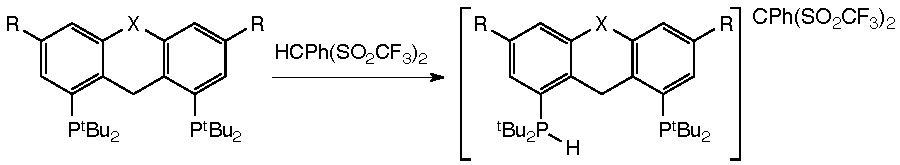
\includegraphics{../Schemes/Protonation.pdf}
\caption[Protonation of the ligands using a strong acid]{Protonation of the ligands using a strong acid}
\label{Protonation}
\end{center}
\end{scheme}

The direct protonation of the ligands using a strong acid resulted in the phosphonium ions shown in Scheme \ref{Protonation}.  \fixme{this data is for the sulfur bridged ligand should I include stuff for silicon as well?}  The \phosphorus{} NMR spectrum has a single broad signal at 15.8 ppm showing a downfield shift of 6.3 ppm upon protonation.  In the \proton{} NMR spectrum the phosphonium proton comes at 9.0~ppm much higher than other phosphonium ions.  In addition the proton appears as an unusual signal in a 1:2:1 ratio with two sharp outer peaks and a broad inner peak.  The \phosphorus{}, \proton{} and \carbon{} spectra show half of the expected peaks indicating a plane of symmetry through the central bridge of the molecule.  However, the signal for the phosphonium proton only integrates for a single proton.  Together with the broadness of the \phosphorus{} and some of the \carbon{} signals indicates a dynamic system in solution with proton exchange between the two phosphorus atoms.  

The degree of dynamism changes between the three ligands.  The sulfur bridged ligand with the smallest bite-angle has the greatest degree of exchange between the systems \fixme{can I get temperatures for coalescence as this would prove it nicely}.  \fixme{the S has the middle one need to check how much coupling in the carbon one}  The sulfur bridged ligand has very little coupling evident in the NMR spectra compared to the silicon bridged ligand which has a number of clearly defined coupled peaks.  The silicon bridged ligand has the largest degree of exchange at room temperature as the phosphorus atoms are held much closer - as shown by the smaller bite-angle which would indicate a greater degree of interaction between the tertiary phosphine and the phosphonium ion and thus much more rapid exchange.  As such at room tempature we are below coalescence and thus the NMR peaks resolve into much clearer signals than those found with the sulfur or carbon bridged systems.

Likewise the carbon bridged system with the largest bite-angle will have the smallest degree of exchange at room temperature.  Hence we are closer to coalescence than in the other two so the NMR spectra are very broad and unable to be fully assigned.  \fixme{check the NMR data for 3013 on 600 MHz}

\fixme{VT NMR data}

Colourless crystals of \fixme{XXX} suitable for X-ray diffraction were grown from the reaction mixture in benzene.  The compound crystallised with two \fixme{molecules} in the unit cell and with benzene solvate, \ce{[StBu-xantphos(H)]CPh(SO2CF3)2}$\cdot{}$ \nicefrac{1}{2}\ce{C6D6} in the monoclinic space group \emph{P}2\sub{1}/\emph{n}. Although the cationic portion was well refined there was significant disorder around the counterion, particularly the \ce{CF3} groups which were refined isotropically as a result. The proton on the phosphonium ion was able to be located and is exclusively located on a single phosphorus atom.  The distances from the proton to the other phosphorus or to the oxygen atom are both too long to indicate any degree of interaction.  \fixme{include stuff about space group etc.}  The crystal structure shows benzene of crystallisation \fixme{check formula} and is consistent as a monoprotonated product.  Important bond lengths are summarised in Table \ref{table:crystalprotonated:lengths} and crystallographic data is given in Table \ref{table:crystalprotonated:data}.

\begin{figure}[h]
\begin{center}
\includegraphics[width=0.8\textwidth]{../Figures/Crystalprotonated.pdf}
\caption[X-ray crystal structure of \ce{[StBu-xantphos(H)]CPh(SO2CF3)2}]{X-ray crystal structure of \ce{[StBu-xantphos(H)]CPh(SO2CF3)2}$\cdot{}$ \nicefrac{1}{2}\ce{C6D6}.  Benzene solvent of crystallisation and hydrogen atoms omitted for clarity}
\label{Crystalprotonated}
\end{center}
\end{figure}

\begin{table}[ht]
\caption[Selected bond distances (\AA) and angles (\degrees) of \ce{StBu-xantphos(H)]CPh(SO2CF3)2}$\cdot{}$ \nicefrac{1}{2}\ce{C6D6}]{Selected bond distances (\AA) and angles (\degrees) of \ce{StBu-xantphos(H)]CPh(SO2CF3)2}$\cdot{}$ \nicefrac{1}{2}\ce{C6D6}} 
\label{table:crystalprotonated:lengths}
\begin{center}
\begin{tabular}{l l l l}
	\toprule
	\multicolumn{2}{l}{\bfseries{~Bond distances (\si{\angstrom})}} & \multicolumn{2}{c}{\bfseries{Bond angles (\degrees)}} \\
	\midrule		
	~P1-H1		~~&~~1.304~~	&~~P1-H1-P1			&~~153.56(7)~~\\	
	~P2-H1		~~&~~2.823~~	&~~P1-O1-P2			&~~86.35(7)~~	\\
	~O-H1		~~&~~2.401~~	&~~~~				&~~~~	\\
	~P1\textprime-H1\textprime~~&~~1.247~~&~~P1\textprime-H1\textprime-P2\textprime&~~158.86(8)~~\\
	~P2\textprime-H1\textprime~~&~~2.935~~&~~P1\textprime-O\textprime-P2\textprime&~~89.23(6)~~\\
	~O\textprime-H1\textprime	~~&~~2.437~~	&~~~~				&~~~~	\\
	\bottomrule{}
\label{table:crystalprotonated:lengths}
\end{tabular}
\end{center}
\end{table}

\begin{table}[htp]
\caption[Crystallographic data of \ce{StBu-xantphos(H)]CPh(SO2CF3)2}$\cdot{}$ \nicefrac{1}{2}\ce{C6D6}]{Crystallographic data of \ce{StBu-xantphos(H)]CPh(SO2CF3)2}$\cdot{}$ \nicefrac{1}{2}\ce{C6D6}} 
\label{table:crystalprotonated:data}
\begin{center}
\begin{tabular}{l l}
	\toprule
	~~\bfseries{Empirical formula}~~&~~\fixme{XXXXX}\\
	\midrule
	~~Formula weight~~		&~~21.8~~	\\
	~~Crystal system~~		&~~24.2~~	\\
	~~Space group~~		&~~20.7~~	\\
	~~a$/$\si{\angstrom}~~	&			\\
	~~b$/$\si{\angstrom}~~	&			\\
	~~c$/$\si{\angstrom}~~	&			\\
	~~$\alpha/$\degrees~~	&			\\
	~~$\beta/$\degrees~~	&			\\
	~~$\gamma/$\degrees~~	&			\\
	~~V$/$\si{\angstrom\cubed}&			\\
	~~Z					&			\\
	~~Cell determination reflections &		\\
	~~Cell determination range, $\theta{}$\textsubscript{min} $\longrightarrow \theta{}$\textsubscript{max}/\degrees &\\
	~~Temperature $/$\si{\kelvin}	&		\\
	~~Radiation type			&		\\
	~~Radiation ($\lambda$) $/$\si{\angstrom}	&	\\
	~~Crystal size $/$\si{\milli\metre}			&	\\
	~~D\textsubscript{\emph{calc}} $/$ \si{\gram\per\metre\cubed}	&	\\
	~~F(000)				&			\\
	~~$\mu /$	\si{\per\milli\metre}		&			\\
	~~Experimental absorption correction type	&	\\
	~~T\textsubscript{max}, T\textsubscript{min}	&	\\
	~~Reflections collected					&	\\
	~~Index range \emph{h}		&		\\
	~~Index range \emph{k}		&		\\
	~~Index range \emph{l}		&		\\
	~~$\theta$ range $/$\degrees	&		\\
	~~Independent reflections		&		\\
	~~Reflections $[\emph{I} > 2\sigma(\emph{I})]$	&	\\
	~~Restraints $/$ parameters	&		\\
	~~GOF					&		\\
	~~R\textsubscript{1} $[\emph{I} > 2\sigma(\emph{I})]$	&	\\
	~~wR2 $[\emph{I} > 2\sigma(\emph{I})]$	&	\\
	~~R\textsubscript{1} [all data]	&		\\
	~~wR2 [all data]			&		\\
	~~Residual density $/$e \si{\per\angstrom\cubed}	&	\\
	\bottomrule
\end{tabular}
\end{center}
\end{table}

\fixme{check that the w in the bottom few rows are not meant to be omegas}
\fixme{something weird going on with alignment fix once the actual table is put in}

The solution and solid-state structures have some distinct differences.  In solution the system is dynamic and has very broad NMR signals particularly in the \phosphorus{} NMR spectrum and has half the number of signals that would be expected in the \proton{}, \phosphorus{} and \carbon{} spectra.  This is likely a result of the rapid exchange of the proton between the two phosphorus atoms resulting in an averaging of the resonances in the NMR spectra.  In the solid state however, the proton occupies a single location which was able to be located from the crystallographic data.  

\fixme{May need to change this as there are two molecules in the asymmetric unit}

\fixme{Check if X-ray should be capitalised}

\fixme{Attempt to react with a deuteron and get a triplet in the phosphorus and changes to the proton} 

\fixme{Check if via should be italicised based on ACS style guide}

\section{Selenides}

Numerous approaches to studying the steric influence of phosphine and diphosphine ligands exist, the most prolific are the Tolman cone angle\cite{Tolman1977} and the natural bite angle\cite{Casey1990} respectively.  The electronic influence are less well defined, typical approaches involve the CO stretching frequency of metal carbonyl complexes or analysis of \oneJPM{} spin-spin coupling constants.  However, the coupling constants are highly dependent on the geometries of metal complexes and this can be influenced significantly be steric constraints, such as those imposed by large diphosphine ligands.  \fixme{footnote? This will be addressed further in \fixme{the complexes chapter}}.  As such the \JPSe{} spin-spin coupling constants of the phosphine selenides is often a more accurate measure of the electronic properties of tertiary phosphines.\cite{Beckmann2011}

The phosphino-selenides are generally relatively straightforward to synthesise and do not require the use of potentially expensive transition metals.  In addition the resulting phosphino-selenides are air-stable as compared to metal carbonyl complexes which often decompose if not stored under carbon monoxide.  The \JPSe{} has shown good correlation with the Tolman electronic parameter.\fixme{find that reference}  In general if the groups on the phosphorus are more electron withdrawing the resulting \JPSe{} increases.  

Phosphorus-selenium coupling constants are not without their restrictions, particularly with diphosphines.  It is not possible to completely eliminate steric influences on the \JPSe{}, selenium has a significant steric and electronic impact resulting in repulsion of the two phosphino-selenides.  This has been noted as the mono- and di-selenides of diphosphines often have different coupling constants.  In these cases the mono-selenide generally gives a better description of the electronic influence of the diphosphine.  

\fixme{Check which order the 1JPM or PSe etc. should be}\\
\fixme{Check if the coupling constants etc. should be hyphenated P-Pt etc. Teresa's paper doesn't}

In addition to the use of \JPSe{} as a measure of the electronic influence of a phosphine it can also be used to measure the Br\o{}nsted basicity of a given phosphine.  A correlation between the experimentally measured \pKb{} and the \JPSe{} has been reported\cite{Beckmann2011} with linear regression: \JPSe{}$ = 7.60 \times{} $ \pKb{} $~+~646~($R$_{2} = 0.9492)$.  As such determining the \JPSe{} allows for calculation of the \pKb{} and has shown good agreement with the experimentally determined data.  \fixme{however it doesn't match well at all for PtBu3 due to changes in the s-character due to steric repulsion}  The \JPSe{} shows solvent dependence just as one would expect for \pKb{} values.  

The ligands \fixme{give references} showed significant resistance to selenation.  Typical methods include heating the phosphine with elemental selenium or reacting with KSeCN.\fixme{citations}  Reaction directly with elemental selenium has been reported as preferable to potassium selenocyanide as the later reacts slowly and gives lower yields.  The allotrope of selenium (red, black or grey) that is utilised is thought not to have an impact on the reaction as both red and black convert to grey upon mild heating.\fixme{get a reference that is not wiki}

The previously reported xantphos selenide was synthesised by refluxing xantphos and red selenium in toluene overnight resulting in diselenation.  Attempting this method with the tBu-xantphos ligands reported here showed little reaction.\fixme{check lab book and NMR as to what happened}  Attempts were also made using KSeCN similar to those previously reported \cite{Bungu2007}.  However, these were also unsuccessful.  Although tBu-xantphos was moderately reactive towards selenium requiring only three days refluxing in toluene, tBu-thixantphos required much longer reaction times will full monoselenation after two weeks at reflux in toluene.  The reason for this may be similar to the effect seen in oxidation.  The sulfur in the backbone has a significant degree of electron density available to interact with the selenium.  Although no selenation at the sulfur was observed \fixme{not sure this is even possible} some degree of \fixme{coordination?} between the sulfur and the selenium may have hindered the reaction resulting in the necessity for much longer reaction times.  

Refluxing the ligands with selenium in toluene for extended periods successfully generated the monoselenated derivative.  Further attempts to diselenate were unsuccessful.  

\fixme{check this data}

The monoselenated tBu-thixantphos derivative was found to have a \JPSe{} = 698.5 Hz, while the monoselenated tBu-xantphos has a \JPSe{} = 696.3 Hz.  These are much lower than that reported for xantphos selenide (749 Hz)\cite{Jahromi2012}.  This lower coupling constant is expected as \emph{tert}-butyl groups are more electron donating than phenyl substituents.  Data for the monoselenated tBu-xantphos derivatives are summarised in Table \ref{table:selenides}.  Upon monoselenation a signal for one of the aromatic protons shifts from 7.60 to 9.26 ppm.   This is likely the proton adjacent to the selected phosphorus as the proximity to the selenium will reduce the shielding on the proton resulting in a downfield chemical shift.\fixme{this seems strange try and find a reference or comparison}

\fixme{find out how to add some space before all tables}

\begin{table}[ht]
\caption[Selected data for the xantphos selenides]{Selected data for the xantphos selenides} 
\label{table:selenides}
\begin{center}
\begin{tabular}{l l l l l l}
	\toprule
	~~Selenide~~ & \multicolumn{2}{c}{$\delta{}$ \phosphorus{} (ppm)} & ~~\JPSe (Hz)~~ & $~~\delta{}$ \selenium{}~~ & ~~\pKb{} ~~\\
	\midrule		
	~~xantphos (diselenide) ~~	&\multicolumn{2}{c}{31.4}		&~~749~~		&~~nr~~	&~~13.55~~\\
	~~tBu-xantphos~~			&~~10.5~~	&~~101.8~~	&~~696.3~~	&~~X~~	&~~6.62~~\\	
	~~tBu-thixantphos~~			&~~X~~	&~~X~~	&~~698.5~~	&~~X~~	&~~6.91~~\\	
	~~tBu-sixantphos~~			&~~X~~	&~~X~~	&~~X~~	&~~X~~	&~~X~~\\	

	\bottomrule{}
\end{tabular}
\end{center}
\end{table}

Using the correlation reported by Beckmann et. al it is possible to convert the \JPSe{} of 698.5 Hz into a \pKb{} of 6.91.  This makes the ligand significantly more basic than xantphos itself with a \pKb{} of 13.55.  The phosphine of closest \pKb{} is \ce{PPhMe2} with a calculated \pKb{} of 8.4 (7.5 experimentally).\fixme{find the original reference}  The two ligands are of considerable similarity however from the \proton{} NMR spectrum of the protonated tBu-thixantphos ligand we can deduce some degree of hydrogen-bonding between the phosphonium ion and the tertiary phosphine.  It is likely that the possibility for this hydrogen-bonding leads to a reduction in the \pKb{} relative to that for \ce{PPhMe2}.  

The tBu-xantphos is more basic than the tBu-thixantphos.  \fixme{why?}  This may be due to sterics \fixme{once I have the value for the silicon I should know more} however it may also be a subtle electronic influence.  Both groups have an ortho ether and a meta alkyl group, in addition tBu-thixantphos has the thioether bridge, thioethers are electron donating by resonance but being in the meta position to the phosphorus the negative charge that could be generated is unable to interact with the phosphorus.  With sulfur being slightly more electronegative than carbon \fixme{reference} a thioether is also slightly inductively electron withdrawing which would result in the phosphorus being very slightly less basic in the tBu-thixantphos case compared to the tBu-xantphos.  




